\documentclass[a4paper,11pt]{ctexart}
\usepackage{amssymb}
\usepackage{amsmath}

\usepackage{graphicx}
\usepackage{geometry}
\geometry{top=2.5cm, bottom=1.8cm, left=2cm, right=2.5cm}
\usepackage{booktabs}
\usepackage{float}

%================ 行距 ================
\usepackage{setspace}
\setstretch{1.3}

\usepackage{calc}
\setlength{\lineskip}{\baselineskip-\ccwd}
\setlength{\lineskiplimit}{2.5pt}

\usepackage{enumitem}
\usepackage{listings}
\lstset{
    basicstyle          =   \sffamily,          % 基本代码风格
    keywordstyle        =   \bfseries,          % 关键字风格
    commentstyle        =   \rmfamily\itshape,  % 注释的风格，斜体
    stringstyle         =   \ttfamily,  % 字符串风格
    flexiblecolumns,                % 别问为什么，加上这个
    numbers             =   left,   % 行号的位置在左边
    showspaces          =   false,  % 是否显示空格，显示了有点乱，所以不现实了
    numberstyle         =   \zihao{-5}\ttfamily,    % 行号的样式，小五号，tt等宽字体
    showstringspaces    =   false,
    captionpos          =   t,      % 这段代码的名字所呈现的位置，t指的是top上面
    frame               =   lrtb,   % 显示边框
}

\renewcommand{\d}{\mathop{}\!\mathrm{d}}
\everymath{\displaystyle}


\begin{document}

\title{微分方程数值解大作业2}
\author{庞逸天 523070910095}
\maketitle

\section{差分格式求解的简要分析}

对于一维对流方程的初值问题：
\[\begin{cases}
    u_t + a u_x = 0, \\
    u(0, x) = f(x) = \begin{cases} 1 & x \le 0, \\ 0 & x > 0 \end{cases}
\end{cases}\]
由于迎风格式、Beam-Warming格式、Lax-Friedrichs格式以及Lax-Wendroff格式均为\textbf{显式差分格式}，在已知初始条件 $u(x,0)$ 的前提下，我们无需求解复杂的线性方程组，可以直接利用第 $n$ 时间层各空间节点的值代数递推计算出第 $n+1$ 时间层的值。

在求解过程中，核心操作是向量化计算，这可以帮助我们减少循环的应用，从而提升计算效率.以迎风格式为例，其显式差分公式为：
    \[ u_j^{n+1} = u_j^n - a\lambda (u_j^n - u_{j-1}^n) \]
    如果使用传统的循环，代码对空间层进行逐点计算：
    \begin{lstlisting}[language=Matlab]
    for j = 2:N_x
        U_uw(j) = U_uw_old(j) - (a*lambda) * (U_uw_old(j) - U_uw_old(j-1));
    end
    \end{lstlisting}
而采用向量化操作后，我们就可以无需使用索引$j$，直接对一整个空间层进行计算。但这时需要注意空间层向量的起始位置和终止位置.由于需要更新的节点范围是 $j \in [2, N_x]$，我们将等式左侧提取为连续的子数组 \texttt{U\_uw(2:end)}。相应地，等式右侧的 $u_j^n$ 对应子数组 \texttt{U\_uw\_old(2:end)}，而空间后退一步的 $u_{j-1}^n$ 则对应子数组 \texttt{U\_uw\_old(1:end-1)}。于是上述逐点循环被等价精简为一行无循环的向量运算：
    \begin{lstlisting}[language=Matlab]
    U_uw(2:end) = U_uw_old(2:end) - (a*lambda) * (U_uw_old(2:end) - U_uw_old(1:end-1));
    \end{lstlisting}
这种将空间层视为整体向量并在每一个时间步内进行同步矩阵更新的方式，极大地减少了Matlab循环语句的开销，提升了计算速度。

\section{算法实现}
基于上述分析，使用Matlab编写四种差分格式求解过程，代码如下：

\begin{lstlisting}[language=Matlab]
%基本参数设置
h = 0.1;                    
tau = 0.08;                
t_end = 4.0;                
N_t = t_end / tau;   
lambda = tau / h;          
x = -4:h:20;               
N_x = length(x);
a_list = [1, 2, 4];

%初始化条件
U0 = zeros(1, N_x);
U0(x <= 0) = 1;

for k = 1:length(a_list)
    a = a_list(k);
    
    %初始化格式的解
    U_uw = U0; 
    U_bw = U0;
    U_lf = U0; 
    U_lw = U0;
    
    % 计算精确解
    U_exact = zeros(1, N_x);
    U_exact((x - a * t_end) <= 0) = 1;
    
    for n = 1:N_t
        U_uw_old = U_uw;
        U_bw_old = U_bw;
        U_lf_old = U_lf;
        U_lw_old = U_lw;
        
        %更新解
        U_uw(2:end) = U_uw_old(2:end) ...
            - (a*lambda) * (U_uw_old(2:end) - U_uw_old(1:end-1));
        U_bw(3:end) = U_bw_old(3:end) ...
            - (a*lambda) * (U_bw_old(3:end) - U_bw_old(2:end-1)) ...
            - 0.5 * (a*lambda) * (1 - (a*lambda)) * ...
            (U_bw_old(3:end) - 2*U_bw_old(2:end-1) + U_bw_old(1:end-2));
        U_lf(2:end-1) = 0.5 * (U_lf_old(3:end) + U_lf_old(1:end-2)) ...
            - 0.5 * (a*lambda) * (U_lf_old(3:end) - U_lf_old(1:end-2));
        U_lw(2:end-1) = U_lw_old(2:end-1) ...
            - 0.5 * (a*lambda) * (U_lw_old(3:end) - U_lw_old(1:end-2)) ...
            + 0.5 * (a*lambda)^2 * ...
            (U_lw_old(3:end) - 2*U_lw_old(2:end-1) + U_lw_old(1:end-2));
        
    end
    
    %绘制图像
    figure('Position', [100, 100, 900, 600]);
    plot(x, U_exact, '-k', 'LineWidth', 2); hold on;
    plot(x, U_uw, '-r', 'LineWidth', 1.5);
    plot(x, U_bw, '-b', 'LineWidth', 1.5);
    plot(x, U_lf, '-g', 'LineWidth', 1.5);
    plot(x, U_lw, '-m', 'LineWidth', 1.5);
    grid on;

    ylim([-0.5, 1.5]);
    xlabel('x');
    ylabel('u');
    title(sprintf('对流方程不同差分格式 (a = %d)', a));
    legend('精确解', '迎风格式 (Upwind)', 'Beam-Warming 格式', ...
           'Lax-Friedrichs 格式', 'Lax-Wendroff 格式', ...
           'Location', 'best', 'FontSize', 11);
end
\end{lstlisting}


\section{数值实验结果与分析}

实验参数为：空间步长 $h=0.1$，时间步长 $\tau=0.08$，终止时间 $t=4.0$，由此可得网格比 $\lambda = \tau/h = 0.8$。

\subsection{当 $a=1$ 时}

此时 $a\lambda = 1 \times 0.8 = 0.8$。计算得到的数值结果如图\ref{fig:a1}所示：

\begin{figure}[H]
    \centering
    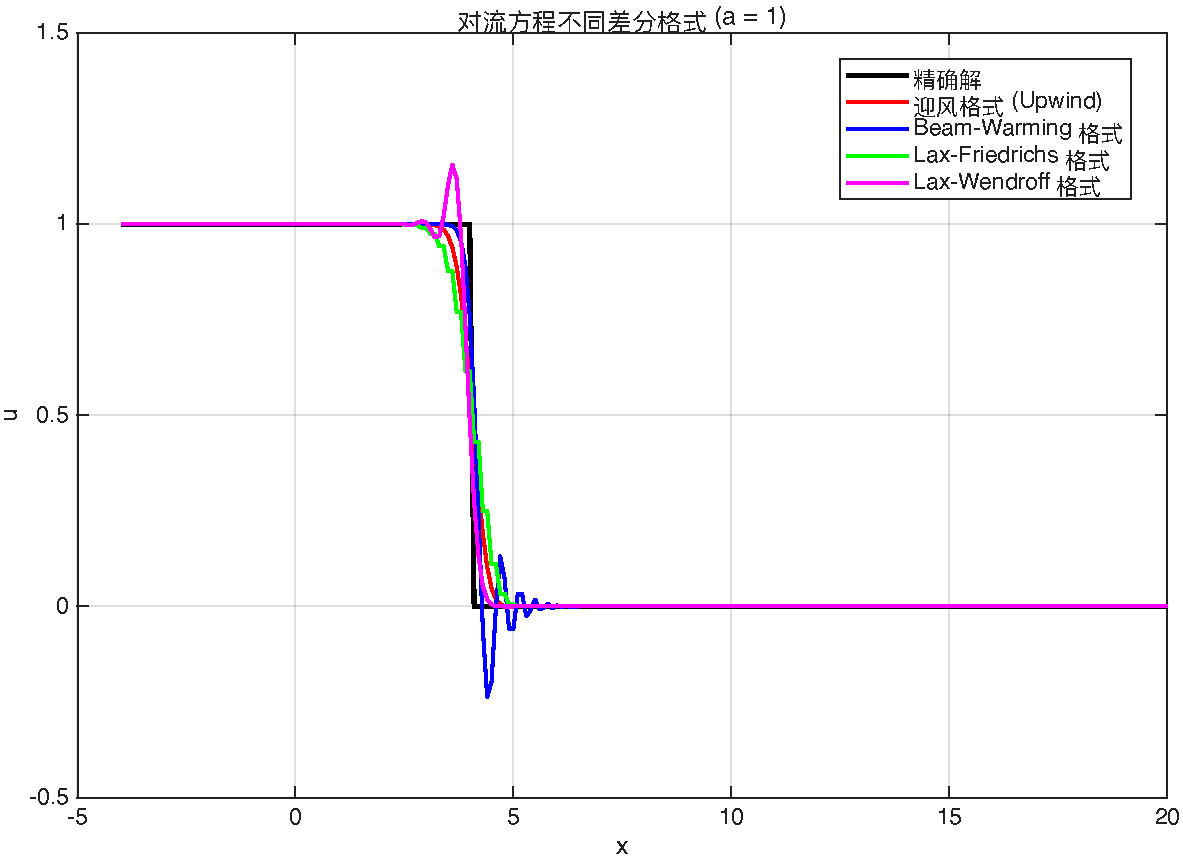
\includegraphics[width=0.9\textwidth]{fig1.pdf}
    \caption{$a=1$ 时四种格式求解结果对比}
    \label{fig:a1}
\end{figure}

从图\ref{fig:a1}中可以观察到：
\begin{enumerate}[label=(\arabic*)]
    \item 在 $a\lambda = 0.8$ 的条件下，四种显式格式均能保持计算的稳定性。
    \item 在间断点附近，\textbf{Lax-Friedrichs格式}出现了非常明显的表现数值耗散.其间断点被大幅抹平，坡度变得极为平缓，且该程度为四种格式中最大的。并且在具体取值中也有明显地阶梯式下降的现象.
    \item \textbf{Beam-Warming格式}和\textbf{Lax-Wendroff格式}分别在在间断点后方和前方出现了较大程度的数值震荡现象，表现为上下波动的振荡。
    \item 相比之下，\textbf{迎风格式}没有出现振荡现象，且下降速度也较为适中，在间断点附近的拟合效果较为平衡。
\end{enumerate}

\vspace{0.5em}
\noindent\textbf{产生不同程度偏差的理论分析：}

对流方程 $u_t + a u_x = 0$ 的物理本质是纯对流过程，不包含耗散（扩散）和色散效应.但在数值离散过程中，由于泰勒展开的截断误差，引入了人为的耗散和色散.
\begin{itemize}
    \item \textbf{Lax-Friedrichs格式与数值耗散}：该格式在时间导数处使用空间平均代替了当前节点值，这在其截断误差中引入了极大的二阶空间导数项，造成了强烈的数值耗散。
    \item \textbf{Lax-Wendroff与Beam-Warming格式}：这两种格式在时空上具有二阶精度，其截断误差的主导项为三阶空间导数项（$u_{xxx}$）。在物理上，三阶导数对应于波的色散效应，在间断点附近形成明显的数值振荡（wiggles）。
    \item \textbf{迎风格式}：作为一阶格式，其截断误差主要也是二阶导数。但相比于LF格式，耗散较小，因此效果适中.
\end{itemize}

\subsection{当 $a=2$ 时}

此时 $a\lambda = 2 \times 0.8 = 1.6$。计算得到的数值结果如图\ref{fig:a2}所示：

\begin{figure}[H]
    \centering
    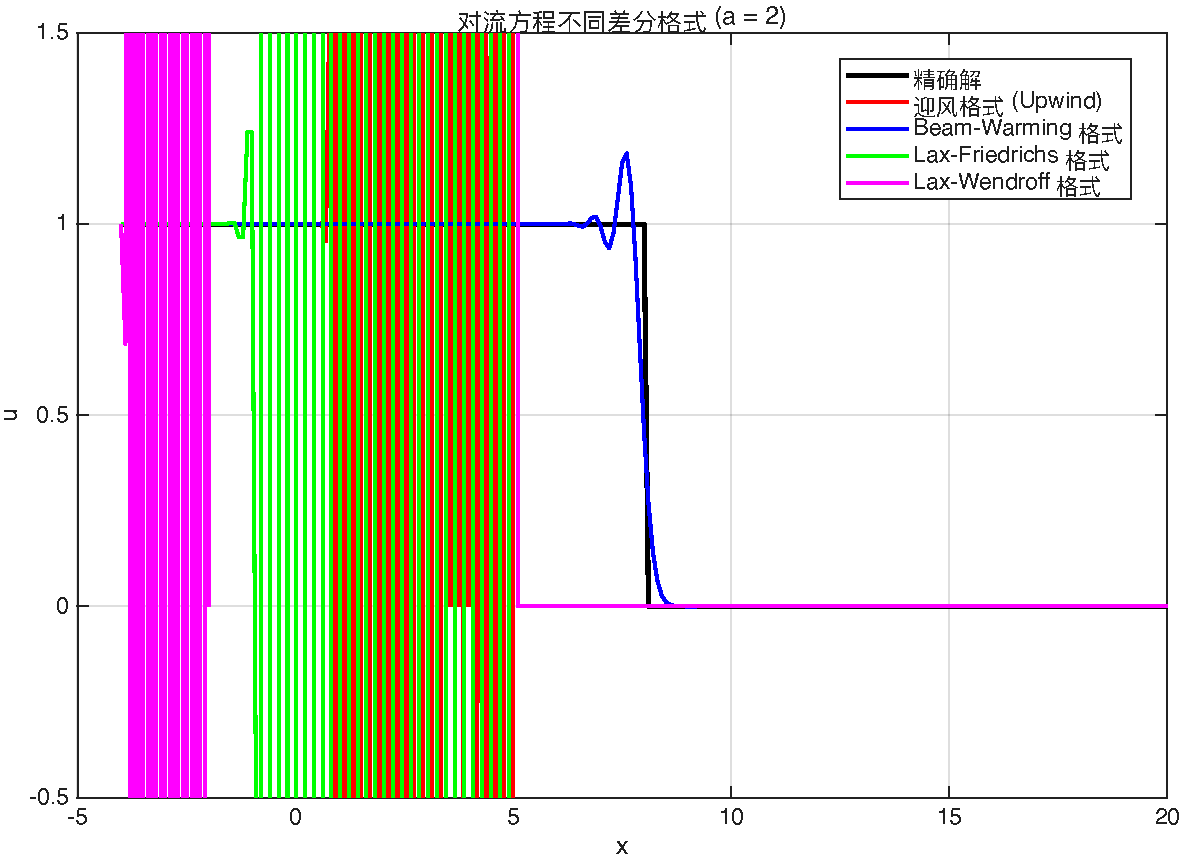
\includegraphics[width=0.9\textwidth]{fig2.pdf}
    \caption{$a=2$ 时四种格式求解结果对比}
    \label{fig:a2}
\end{figure}

由图\ref{fig:a2}明显可见，当 $a\lambda$ 的值增大到 $1.6$ 后，原先均能稳定求解的差分格式表现出了极大的差异：
除了\textbf{Beam-Warming格式}依旧能够保持收敛且伴随一定程度的振荡外，迎风格式、Lax-Friedrichs格式和Lax-Wendroff格式均发生了极其严重的数值发散，无法得到具有任何物理意义的解。

\subsection{当 $a=4$ 时}

此时 $a\lambda = 4 \times 0.8 = 3.2$。计算得到的数值结果如图\ref{fig:a3}所示：

\begin{figure}[H]
    \centering
    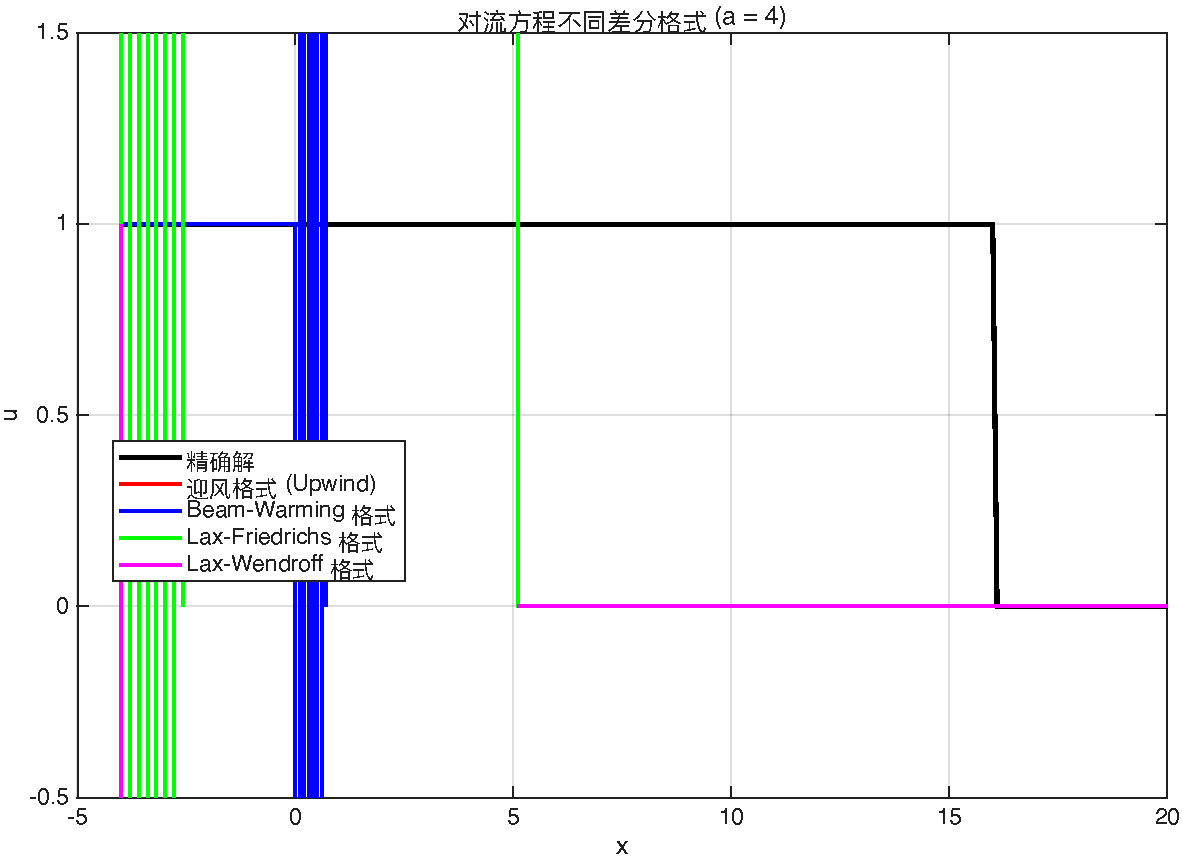
\includegraphics[width=0.9\textwidth]{fig3.pdf}
    \caption{$a=4$ 时四种格式求解结果对比}
    \label{fig:a3}
\end{figure}

从图\ref{fig:a3}中可以发现，随着参数的进一步增大到 $a\lambda = 3.2$，即便是在 $a=2$ 时表现出稳定性的 Beam-Warming 格式也丧失了稳定性。四种差分算法在此参数下均呈现出发散状态。


\section{数值分析：CFL条件与稳定性分析}

理论上，我们可以使用\textbf{CFL条件}解释上述不同参数下差分格式发散或稳定的现象.

\subsection{CFL条件简介}
CFL条件是显式数值方法能够收敛的必要条件.通过Von Neumann稳定性分析法或是绘制图像，我们可以推导出题目中所使用的四种显式差分格式的理论稳定条件：
\begin{itemize}
    \item 迎风格式的稳定条件：$0 \le a\lambda \le 1$
    \item Lax-Friedrichs格式的稳定条件：$|a\lambda| \le 1$
    \item Lax-Wendroff格式的稳定条件：$|a\lambda| \le 1$
    \item Beam-Warming格式的稳定条件：$0 \le a\lambda \le 2$
\end{itemize}

利用CFL条件的理论极限，能够完美地解释本次实验的测试结果：
\begin{itemize}
    \item 当 $a=1$ 时，$a\lambda = 0.8$。此时 $a\lambda$ 均小于所有格式的稳定上限，故四种方法全部稳定。
    \item 当 $a=2$ 时，$a\lambda = 1.6$。此时 $1.6 > 1$，迎风、LF和LW格式均突破了稳定极限，发生发散；而 Beam-Warming 的稳定上限为 $2$，因此在此参数下它是唯一保持稳定的格式。
    \item 当 $a=4$ 时，$a\lambda = 3.2$。此时不仅突破了 $1$，也突破了 Beam-Warming 的极限 $2$，因此四种格式完全发散。
\end{itemize}

\end{document}